\section{Crohn's Disease}
Crohn's Disease \cite{baumgart2012crohn,crohnsNHS} is one of the primary types of Inflammatory Bowel Disease (IBD) \cite{IBDCDC}. It is characterised by its chronic nature with inflammation in the gastrointestinal (GI) tract (indicated in \autoref{fig:gi-tract} \cite{digestio98:online}). This condition can lead to long-term damage and complications, such as strictures, fistulas, and abscesses. Many people worldwide struggle with IBD, and the management remains challenging for medical professionals to address. A study from the University of Nottingham \cite{UoNResearch} reports that more than half a million individuals in the UK are affected by Crohn's Disease and Ulcerative Colitis, another significant IBD subtype. 

Unlike Ulcerative Colitis, which is limited to the colon and rectum, Crohn's disease can potentially develop lesions anywhere within the GI tract. Consequently, patients may experience diverse symptoms, including abdominal pain, diarrhoea, fatigue, and weight loss.
\begin{figure}[htp]
    \centering
    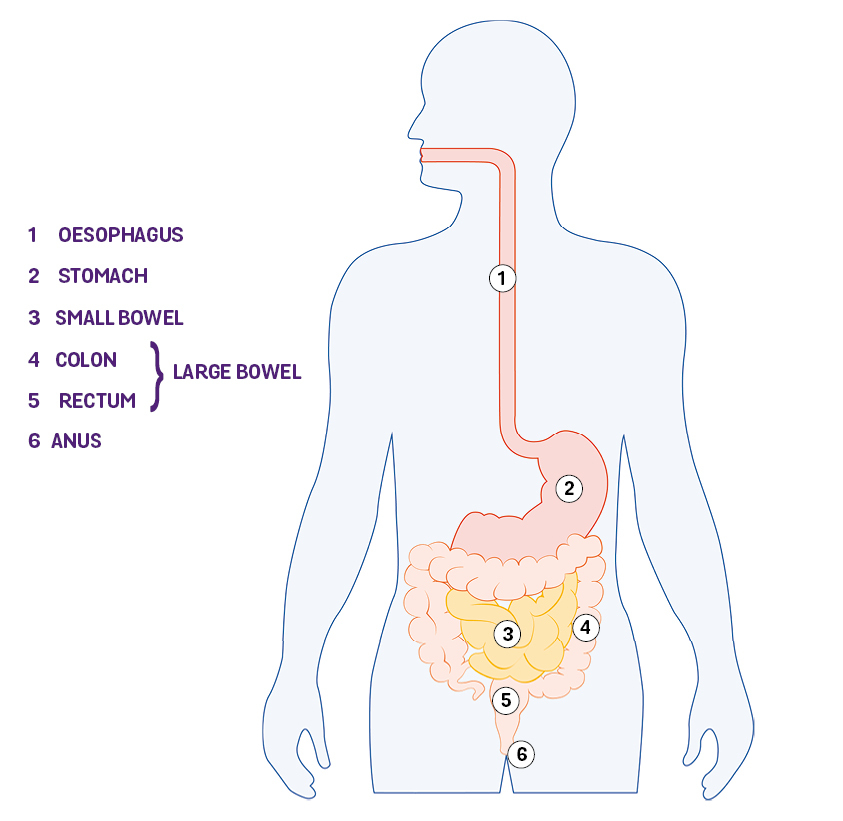
\includegraphics[width=0.5\textwidth]{figures/digestion-graphic.jpg}
    \caption{The gastrointestinal tract of a Human}
    \label{fig:gi-tract}
\end{figure}

Although numerous research initiatives have been undertaken \cite{hoarau2016bacteriome,feuerstein2021aga}, the precise cause of Crohn's disease is still not wholly understood, rendering it incurable. However, fortunately, early diagnosis and appropriate treatment can alleviate patients' symptoms and substantially improve their quality of life. Various diagnostic methods are employed by clinicians, such as enteroclysis, endoscopy, colonoscopy, and radiographic techniques (including barium contrast X-rays, Computed Tomography (CT), and Magnetic Resonance Imaging (MRI)) to assist in the early diagnosis of the disease. MRI has become increasingly popular among radiographic techniques due to its non-invasive nature and enhanced imaging capabilities compared to CT. Nevertheless, manual MRI scan analysis remains a challenge since it is a time-consuming and labour-intensive process. Additionally, medical experts must examine each scan slice by slice painstakingly.

\section{Motivation}

The advancement of Machine Learning and Deep Learning technologies, notably Convolutional Neural Networks (CNNs), offers powerful means for automatic feature extraction from image data and supporting medical professionals in diagnostic tasks. One crucial aspect of Crohn's Disease diagnosis is the examination of the terminal ileum (T.I.). Holland et al.'s study \cite{holland2019automatic} in 2019 proposed a residual network specifically targeting the terminal ileum to facilitate automated detection of Crohn's Disease using MRI scans. The authors claimed that the efficacy of their framework was contingent upon the degree of localisation during the preprocessing stage. Consequently, they advocated for incorporating terminal ileal ground-truth segmentations to enhance the localisation of the terminal ileum and improve the performance of automated detection techniques.

In a subsequent study, Abidi et al. \cite{Ali2022} advanced this line of research by developing an innovative deep-learning segmentation based on semi-supervised learning techniques and the nnU-Net architecture \cite{isensee2021nnu}. This approach utilised the centerline coordinates of the critical region to augment the data during training time, thus enabling the automatic localisation of critical regions. Abidi et al.'s research mainly focus on the localisation terminal ileum, which is essential for radiologists during diagnostic assessments. The researchers addressed the previously identified limitations regarding the high dependence on localisation during the preprocessing phase \cite{holland2019automatic}. Furthermore, their findings established a solid foundation for a multi-class terminal ileum segmentation algorithm that combines transfer learning strategies with the nnU-Net architecture.

Inspired by the insights from \cite{holland2019automatic, Ali2022}, this project aims to continue the work performed by \cite{Ali2022}, leveraging advanced deep-learning techniques to enhance the segmentation performance of the terminal ileum in MRI scans. The successful accomplishment of this objective will significantly aid clinicians in diagnosing Crohn's disease, ultimately contributing to enhanced patient outcomes.

\section{Machine Learning Challenges}

The efficacy of deep learning models is intrinsically linked to the training data's quality, quantity, and diversity. One of the principal challenges faced in this project is the limited availability of training data. The dataset at our disposal is relatively small, comprising only 233 patient cases for three modalities of MRI scans, which pales compared to those utilised in other industry-leading deep learning systems. 

Our image data's region of interest (ROI) occupies a minor portion of the MRI scan. Additional preprocessing techniques, such as bounding box localisation and cropping, must be considered for enhancing the segmentation model's performance, as suggested by \cite{Ali2022}. Another major challenge is the necessity for manual segmentation by clinical experts to develop gold-standard labels or point-wise centerlines for patient data. This is indeed a complex, laborious, and inefficient endeavour. Consequently, acquiring high-quality and abundant patient data and gold-standard annotations poses significant challenges.

To mitigate these concerns, we propose a proxy training task employing weak supervision to generate coarse-grained segmentation masks as a compromise for the scarcity of gold-standard segmentations. Upon completion of the proxy task, gold-standard segmentations will be integrated into the training process to produce the final segmentation model. Prior also research \cite{Ali2022} indicates that implementing transfer learning for proxy training \cite{jang2021effectiveness} or incorporating a related pre-training job may serve as potential solutions to address these limitations.

\section{Objectives}

This project uses deep learning methodologies to construct an enhanced terminal ileum segmentation model based on prior work. To achieve this, we will solidify the previous research as a firm foundation and then incorporate sophisticated transfer and semi-supervised learning techniques. The specific objectives that inform our strategic approach include:

\begin{itemize}

\item We aim to establish a nnU-Net-based baseline segmentation model from the based prior work. The model training includes a proxy task and a fine-tuning task. In the proxy task, we propose generating coarse-grained weak masks with centerline coordinates of the critical region with Simple Linear Iterative Clustering (SLIC) method for data without ground-truth annotations. These masks serve as a foundation for establishing the proxy training task. After training the proxy model using the generated weak masks, we plan to use the proxy model in conjunction with fully annotated data to develop our target segmentation model. This target model will set the baseline for subsequent refinement.
\item Once our baseline is set, we plan to have another approach to generate weak masks in the proxy task by utilising the pre-trained SegmentAnything Model \cite{kirillov2023segany} from Meta AI. We will work on its medical imaging variant, MedSAM and fine-tune the model with our dataset. After fine-tuning, we can use the MedSAM model to generate weak masks, using the weak masks to complete the proxy task and obtain a refined model with full supervision.

\item An essential part of our project is monitoring and quantitatively evaluating the performance of all developed models. We will compare the Dice Similarity Coefficient (DSC) to assess the quality of generated weak masks and the final segmentation performance between the baseline and our refined model. Additional statistical tests, such as t-test or f-test, will be applied to validate the statistical significance of our model's performance. To investigate the effect of possible critical components for the model training, ablation studies will be performed to analyse the importance of elements in the training trajectory. 
\end{itemize}